%-----------------------------------------------------------------------------------------------------------------------------------------------%
%	The MIT License (MIT)
%
%	Copyright (c) 2019 Jan Küster
%
%	Permission is hereby granted, free of charge, to any person obtaining a copy
%	of this software and associated documentation files (the "Software"), to deal
%	in the Software without restriction, including without limitation the rights
%	to use, copy, modify, merge, publish, distribute, sublicense, and/or sell
%	copies of the Software, and to permit persons to whom the Software is
%	furnished to do so, subject to the following conditions:
%	
%	THE SOFTWARE IS PROVIDED "AS IS", WITHOUT WARRANTY OF ANY KIND, EXPRESS OR
%	IMPLIED, INCLUDING BUT NOT LIMITED TO THE WARRANTIES OF MERCHANTABILITY,
%	FITNESS FOR A PARTICULAR PURPOSE AND NONINFRINGEMENT. IN NO EVENT SHALL THE
%	AUTHORS OR COPYRIGHT HOLDERS BE LIABLE FOR ANY CLAIM, DAMAGES OR OTHER
%	LIABILITY, WHETHER IN AN ACTION OF CONTRACT, TORT OR OTHERWISE, ARISING FROM,
%	OUT OF OR IN CONNECTION WITH THE SOFTWARE OR THE USE OR OTHER DEALINGS IN
%	THE SOFTWARE.
%	
%
%-----------------------------------------------------------------------------------------------------------------------------------------------%

\documentclass[10pt,A4]{article}  

%----------------------------------------------------------------------------------------
% ENCODING
%----------------------------------------------------------------------------------------
% Remove blank pages
\let\clearpage\relax

% we use utf8 since we want to build from any machine
\usepackage[utf8]{inputenc}   

%----------------------------------------------------------------------------------------
% LOGIC
%----------------------------------------------------------------------------------------

% provides \isempty test
\usepackage{xstring, xifthen}

%----------------------------------------------------------------------------------------
% FONT BASICS
%----------------------------------------------------------------------------------------

% some tex-live fonts - choose your own

%\usepackage[defaultsans]{droidsans}
%\usepackage[default]{comfortaa}
%\usepackage{cmbright}
\usepackage[default]{raleway}
%\usepackage{fetamont}
%\usepackage[default]{gillius}
%\usepackage[light,math]{iwona}
%\usepackage[thin]{roboto} 

% set font default
\renewcommand*\familydefault{\sfdefault}  
\usepackage[T1]{fontenc}

% more font size definitions
\usepackage{moresize}
%----------------------------------------------------------------------------------------
% FONT AWESOME ICONS
%---------------------------------------------------------------------------------------- 

% include the fontawesome icon set
\usepackage{fontawesome}

% use to vertically center content
% credits to: http://tex.stackexchange.com/questions/7219/how-to-vertically-center-two-images-next-to-each-other
\newcommand{\vcenteredinclude}[1]{\begingroup
\setbox0=\hbox{\includegraphics{#1}}%
\parbox{\wd0}{\box0}\endgroup}

% use to vertically center content
% credits to: http://tex.stackexchange.com/questions/7219/how-to-vertically-center-two-images-next-to-each-other
\newcommand*{\vcenteredhbox}[1]{\begingroup
\setbox0=\hbox{#1}\parbox{\wd0}{\box0}\endgroup}

% icon shortcut
\newcommand{\icon}[3] {               
  \makebox(#2, #2){\textcolor{maincol}{\csname fa#1\endcsname}}
} 

% icon with text shortcut
\newcommand{\icontext}[4]{            
  \vcenteredhbox{\icon{#1}{#2}{#3}}  \hspace{2pt}  \parbox{0.9\mpwidth}{\textcolor{#4}{#3}}
}

% icon with website url
\newcommand{\iconhref}[5]{            
    \vcenteredhbox{\icon{#1}{#2}{#5}}  \hspace{2pt} \href{#4}{\textcolor{#5}{#3}}
}

% icon with email link
\newcommand{\iconemail}[5]{             
    \vcenteredhbox{\icon{#1}{#2}{#5}}  \hspace{2pt} \href{mailto:#4}{\textcolor{#5}{#3}}
}

%----------------------------------------------------------------------------------------
% PAGE LAYOUT  DEFINITIONS
%----------------------------------------------------------------------------------------

% page outer frames (debug-only)
% \usepackage{showframe}    

% we use paracol to display breakable two columns
\usepackage{paracol}

% define page styles using geometry
\usepackage[a4paper]{geometry}

% remove all possible margins
\geometry{top=1cm, bottom=1cm, left=1cm, right=1cm}

\usepackage{fancyhdr}
\pagestyle{empty}

% space between header and content
% \setlength{\headheight}{0pt}

% indentation is zero
\setlength{\parindent}{0mm}

%----------------------------------------------------------------------------------------
% TABLE /ARRAY DEFINITIONS
%---------------------------------------------------------------------------------------- 

% extended aligning of tabular cells
\usepackage{array}

% custom column right-align with fixed width
% use like p{size} but via x{size}
\newcolumntype{x}[1]{%
>{\raggedleft\hspace{0pt}}p{#1}}%


%----------------------------------------------------------------------------------------
% GRAPHICS DEFINITIONS
%---------------------------------------------------------------------------------------- 

%for header image
\usepackage{graphicx}

% use this for floating figures
% \usepackage{wrapfig}
% \usepackage{float}
% \floatstyle{boxed} 
% \restylefloat{figure}

%for drawing graphics   
\usepackage{tikz}       
\usetikzlibrary{shapes, backgrounds,mindmap, trees}

%----------------------------------------------------------------------------------------
% Color DEFINITIONS
%---------------------------------------------------------------------------------------- 
\usepackage{transparent}
\usepackage{color}

% primary color
\definecolor{maincol}{RGB}{ 225, 0, 0 }

% accent color, secondary
% \definecolor{accentcol}{RGB}{ 250, 150, 10 }

% dark color
\definecolor{darkcol}{RGB}{ 70, 70, 70 }

% light color
\definecolor{lightcol}{RGB}{245,245,245}


% Package for links, must be the last package used
\usepackage[hidelinks]{hyperref}
\hypersetup{
    colorlinks=true,
    linkcolor=maincol,
    urlcolor=maincol,
}

% returns minipage width minus two times \fboxsep
% to keep padding included in width calculations
% can also be used for other boxes / environments
\newcommand{\mpwidth}{\linewidth-\fboxsep-\fboxsep}
  


%============================================================================%
%
% CV COMMANDS
%
%============================================================================%

%----------------------------------------------------------------------------------------
%  CV LIST
%----------------------------------------------------------------------------------------

% renders a standard latex list but abstracts away the environment definition (begin/end)
\newcommand{\cvlist}[1] {
  \begin{itemize}{#1}\end{itemize}
}

%----------------------------------------------------------------------------------------
%  CV TEXT
%----------------------------------------------------------------------------------------

% base class to wrap any text based stuff here. Renders like a paragraph.
% Allows complex commands to be passed, too.
% param 1: *any
\newcommand{\cvtext}[1] {
  \begin{tabular*}{1\mpwidth}{p{0.98\mpwidth}}
    \parbox{1\mpwidth}{#1}
  \end{tabular*}
}

%----------------------------------------------------------------------------------------
% CV SECTION
%----------------------------------------------------------------------------------------

% Renders a a CV section headline with a nice underline in main color.
% param 1: section title
\newcommand{\cvsection}[1] {
  \vspace{14pt}
  \cvtext{
    \textbf{\LARGE{\textcolor{darkcol}{\uppercase{#1}}}}\\[-4pt]
    \textcolor{maincol}{ \rule{0.1\textwidth}{2pt} } \\
  }
}

%----------------------------------------------------------------------------------------
% META SKILL
%----------------------------------------------------------------------------------------

% Renders a progress-bar to indicate a certain skill in percent.
% param 1: name of the skill / tech / etc.
% param 2: level (for example in years)
% param 3: percent, values range from 0 to 1
\newcommand{\cvskill}[3] {
  \begin{tabular*}{1\mpwidth}{p{0.72\mpwidth}  r}
    \textcolor{black}{\textbf{#1}} & \textcolor{maincol}{#2}\\
  \end{tabular*}%
  
  \hspace{4pt}
  \begin{tikzpicture}[scale=1,rounded corners=2pt,very thin]
    \fill [lightcol] (0,0) rectangle (1\mpwidth, 0.15);
    \fill [maincol] (0,0) rectangle (#3\mpwidth, 0.15);
    \end{tikzpicture}%
}


%----------------------------------------------------------------------------------------
%  CV EVENT
%----------------------------------------------------------------------------------------

% Renders a table and a paragraph (cvtext) wrapped in a parbox (to ensure minimum content
% is glued together when a pagebreak appears).
% Additional Information can be passed in text or list form (or other environments).
% the work you did
% param 1: time-frame i.e. Sep 14 - Jan 15 etc.
% param 2:   event name (job position etc.)
% param 3: Customer, Employer, Industry
% param 4: Short description
% param 5: work done (optional)
% param 6: technologies include (optional)
% param 7: achievements (optional)
\newcommand{\cvevent}[7] {

  % we wrap this part in a parbox, so title and description are not separated on a pagebreak
  % if you need more control on page breaks, remove the parbox
  
    \begin{tabular*}{1\mpwidth}{p{0.72\mpwidth}  r}
      \textcolor{black}{\textbf{#2}} & \colorbox{maincol}{\makebox[0.25\mpwidth]{\textcolor{white}{#1}}} \\
      \textcolor{maincol}{\textbf{#3}} & \\
    \end{tabular*}\\[1pt]
  
    \ifthenelse{\isempty{#4}}{}{
      \cvtext{#4}\\
    }
  \ifthenelse{\isempty{#5}}{}{
    \vspace{9pt}
    {#5}
  }
  % \vspace{14pt}
}

%----------------------------------------------------------------------------------------
%  CV META EVENT
%----------------------------------------------------------------------------------------

% Renders a CV event on the sidebar
% param 1: title
% param 2: subtitle (optional)
% param 3: customer, employer, etc,. (optional)
% param 4: info text (optional)
\newcommand{\cvmetaevent}[4] {
  \textcolor{maincol} 
  {\cvtext{
    \vspace{-10pt}
  \textbf{\begin{flushleft}#1\end{flushleft}}}}

  \ifthenelse{\isempty{#2}}{}{
    \vspace{-5pt}
  \textcolor{darkcol} {\cvtext{\textbf{#2}} }
  }

  \ifthenelse{\isempty{#3}}{}{
    \cvtext{{ \textcolor{darkcol} {#3} }}\\
    \vspace{-10pt}
  }

  \cvtext{#4}\\[14pt]
}

%============================================================================%
%
%
%
% DOCUMENT CONTENT
%
%
%
%============================================================================%
\begin{document}
\columnratio{0.31}
\setlength{\columnsep}{2.2em}
\setlength{\columnseprule}{4pt}
\colseprulecolor{lightcol}
\begin{paracol}{2}
\begin{leftcolumn}
  %---------------------------------------------------------------------------------------
  % META IMAGE
  %----------------------------------------------------------------------------------------
  % \begin{center}
  % 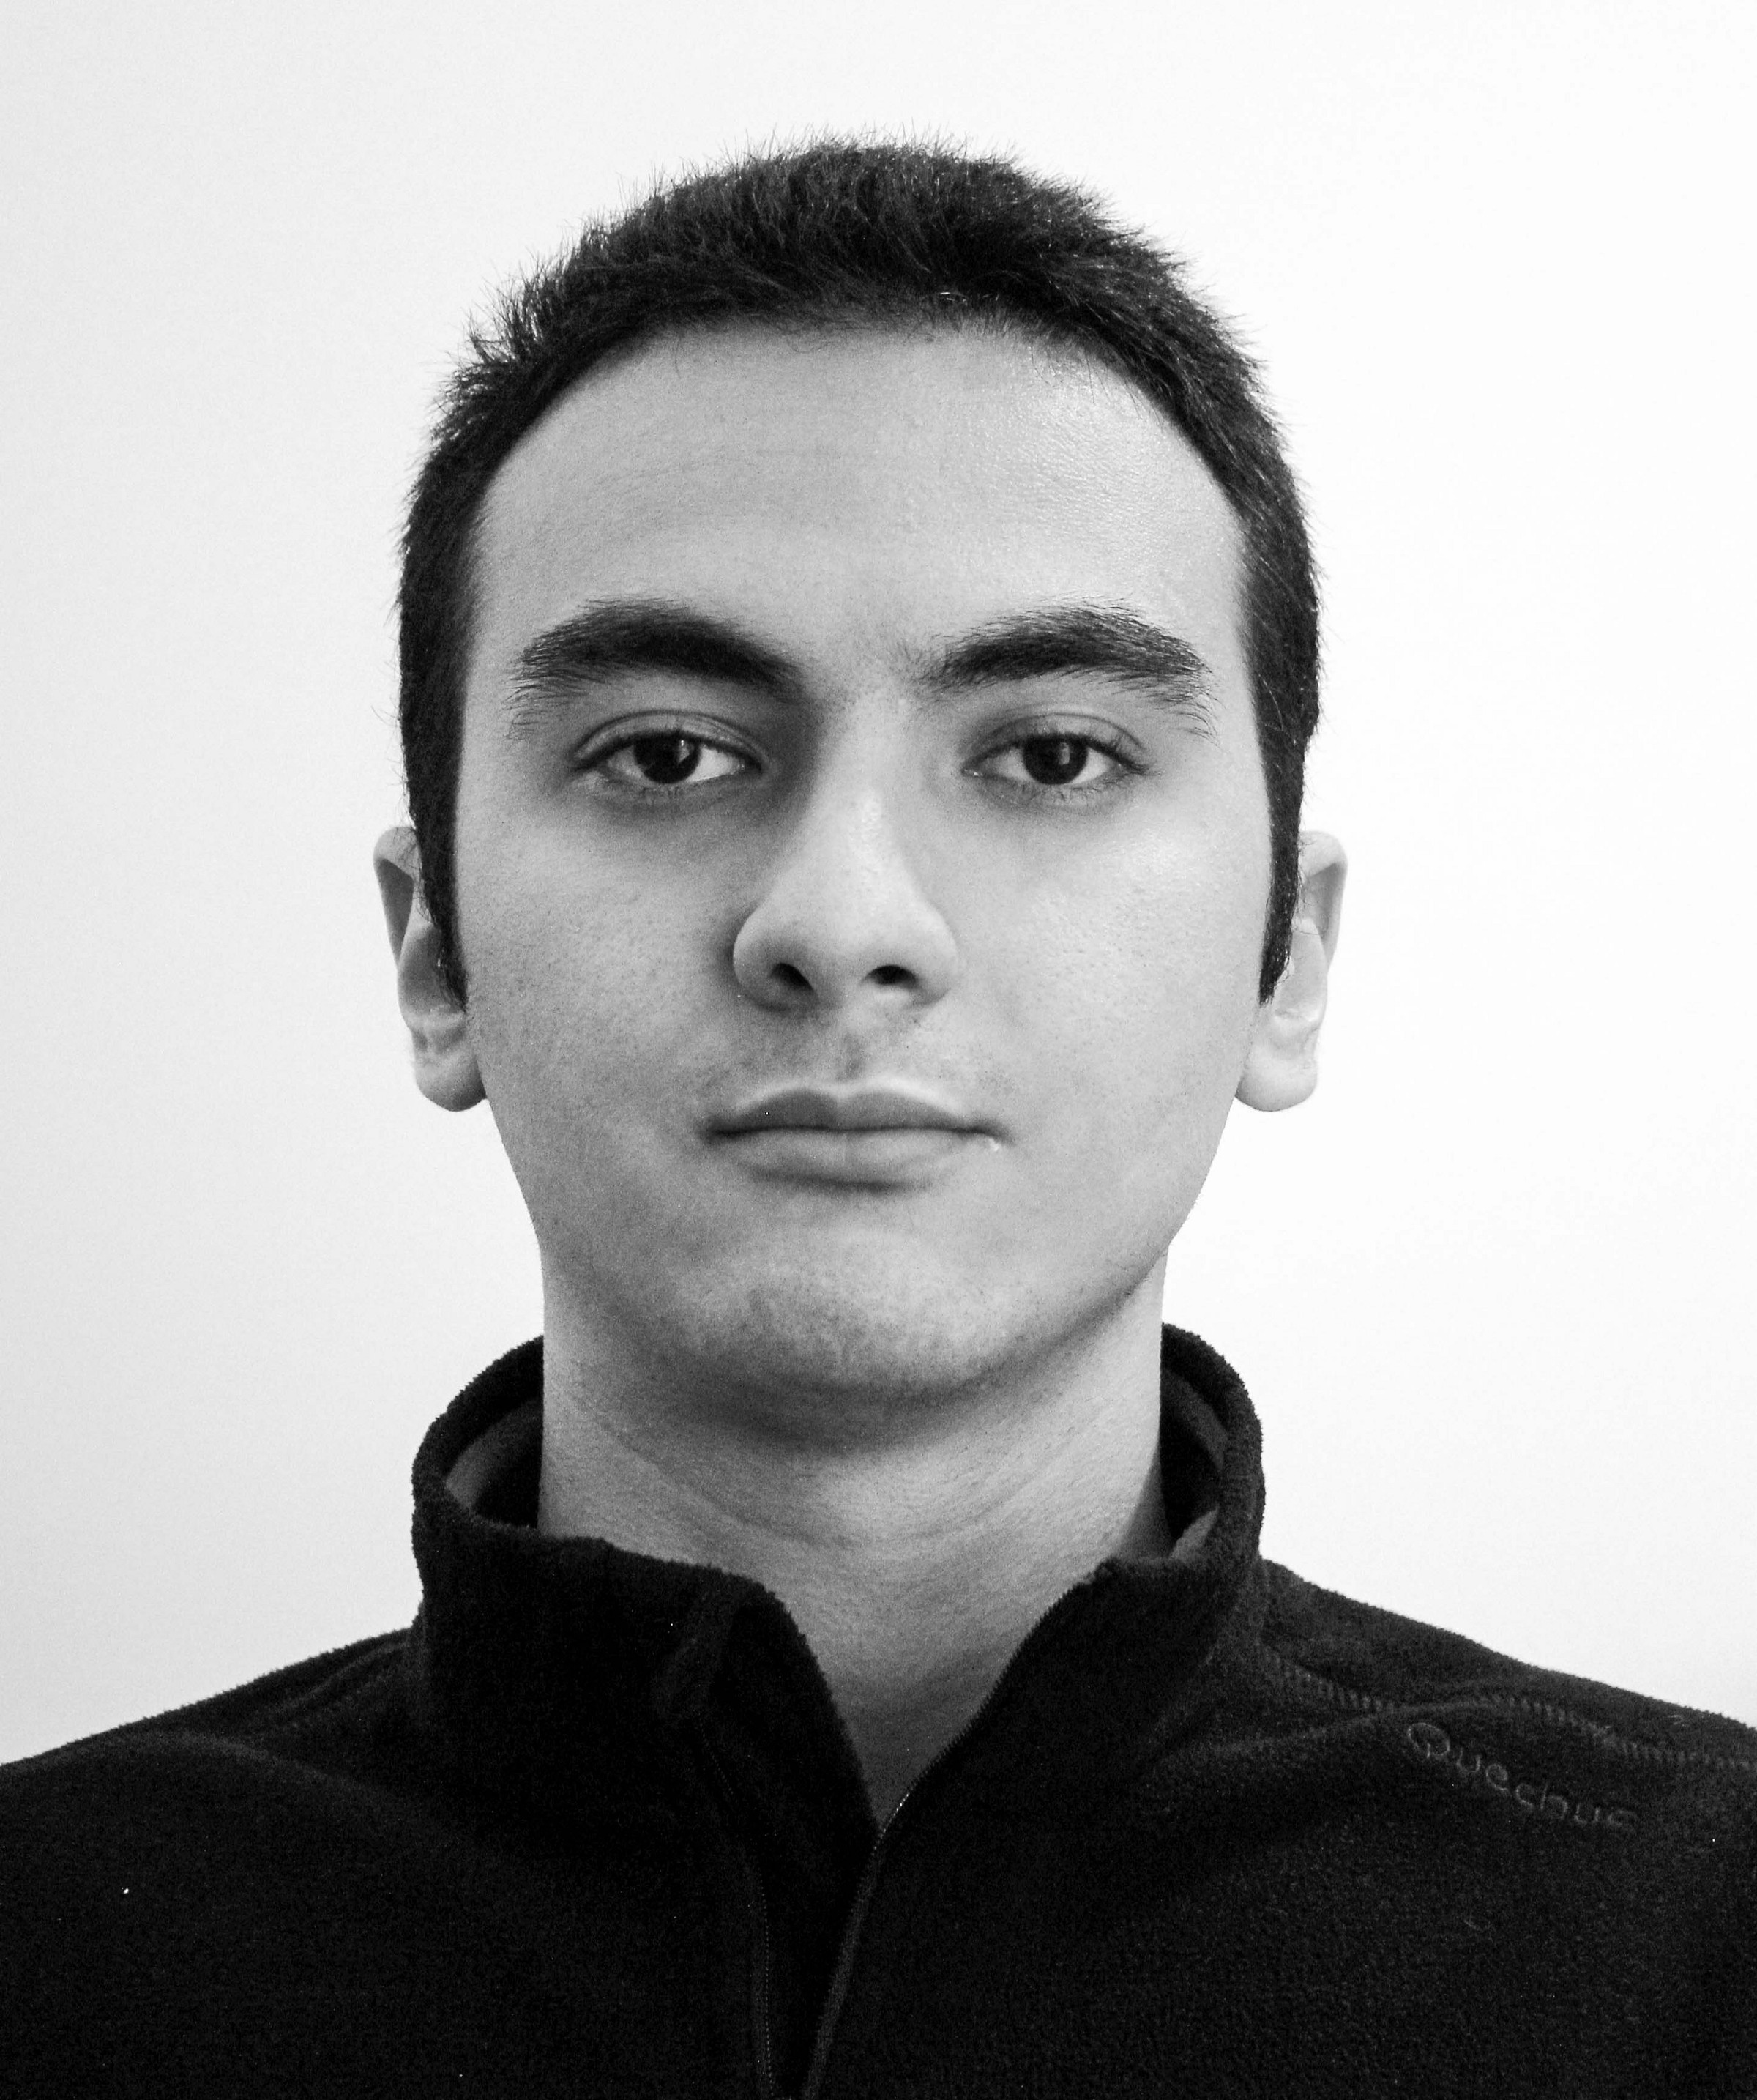
\includegraphics[width=90pt,height=110pt]{Yousef.jpeg} 
  % \end{center}
  \begin{center}
  
\includegraphics[width=100pt,height=100pt]{majhoolsoft.com QRcode.png} 
  \end{center}
  %trimming relative to image size
  %---------------------------------------------------------------------------------------
  % EDUCATION
  %----------------------------------------------------------------------------------------
  \cvsection{EDUCATION}
  \cvmetaevent{2014 - 2019}
  {B. Sc. Computer Engineering.}
  {\href{https://aut.ac.ir/en}{
  \small{Amirkabir University of Technology}}\\
  \small{(Tehran Polytechnic)}\\
  }
  {Advisor: \href{https://www.torontomu.ca/information-technology-management/faculty-research/mehdi-shajari/}{Dr. Mehdi Shajari}}
\\
  %---------------------------------------------------------------------------------------
  % META SKILLS
  %----------------------------------------------------------------------------------------
  \cvsection{SKILLS}
    
  \vspace{-10pt}
    
  \cvskill{HTML/CSS/SCSS} {3+ yrs} {0.85} \\[-2pt]

  \cvskill{JavaScript} {2+ yrs} {0.7} \\[-2pt]

  \cvskill{PHP} {2+ yrs} {0.6} \\[-2pt]

  \cvskill{SQL/No-SQL} {2+ yrs} {0.6} \\[-2pt]

  \cvskill{UI Design Tools} {2+ yrs} {0.6} \\[-2pt]

  \cvskill{Linux} {2+ yrs} {0.5} \\[-2pt]

  \cvskill{Unit Test} {1- yrs} {0.3} \\[-2pt]

  \cvskill{REST API/GraphQL} {2+ yrs} {0.5} \\[-2pt]

  \cvskill{Cloud Computing} {1- yrs} {0.3} \\[-2pt]

  \cvskill{GIT} {3+ yrs} {0.65} \\[-2pt]
%---------------------------------------------------------------------------------------
% Contact
%----------------------------------------------------------------------------------------

\cvsection{CONTACT}

  \icontext{MapMarker}{12}{Calgary, Alberta}{black}\\[6pt]
  \icontext{Phone}{12}{587 897 3048 }{black}\\[6pt]
  \iconhref{Globe}{12}{\color{maincol}{Majhoolsoft.github.io}}{https://majhoolsoft.github.io}{black}\\[6pt]
  \iconemail{Envelope}{12}{\color{maincol}{fatouraee96@gmail.com}}{fatouraee96@gmail.com}{black}\\[6pt]
  \iconhref{File}{12}{\color{maincol}{Medium}}{https://medium.com/@majhoolsoft}{black}\\[6pt]
  \iconhref{Linkedin}{12}{\color{maincol}{Linked In}}{https://www.linkedin.com/in/yousef-fatouraee/}{black}\\[6pt]
  \iconhref{Youtube}{12}{\color{maincol}{YouTube}}{https://www.youtube.com/@majhoolsoft}{black}\\[6pt]
  \\
\end{leftcolumn}
\begin{rightcolumn}
%---------------------------------------------------------------------------------------
% TITLE  HEADER
%----------------------------------------------------------------------------------------
\fcolorbox{white}{darkcol}{\begin{minipage}[c][2.2cm][c]{1\mpwidth}
  \begin {center}
  \Huge{ \textbf{ \textcolor{white}{ \uppercase{ Yousef Fatouraee } } } } \\[-24pt]
  \textcolor{white}{ \rule{0.1\textwidth}{1.25pt} } \\[4pt]
  \large{ \textcolor{white} {Software Engineer} }
  \end {center}
  \end{minipage}} \\[14pt]
\vspace{-20pt}
%---------------------------------------------------------------------------------------
% SUMMARY
%----------------------------------------------------------------------------------------

\cvsection{SUMMARY}

\cvtext{Self-taught and motivated \textbf{Web Developer}
  with 2+ years of experience.\\
  Skilled in \textbf{HTML, CSS, JavaScript}, and familiar with \textbf{Front-end} libraries such as \textbf{React.js}, \textbf{Vue.js}, and \textbf{jQuery}.
}

%---------------------------------------------------------------------------------------
% WORK EXPERIENCE
%----------------------------------------------------------------------------------------
\cvsection{WORK EXPERIENCE}

\cvevent
{July 19 - July 21}
{Imen Rayaneh Amirkabir}
{Web Developer}
{\cvlist{
          % \item{
          %       Actively engaged in web creative  \textbf{design}
          % }
          \item{
                Developed responsive  \textbf{UI} using \textbf{imperative JS}, \textbf{HTML5} and \textbf{CSS3} by translating \textbf{sketches} and \textbf{wireframes} into high-quality code and engaging in web creative \textbf{design}
          }\item{
                Developed \textbf{portal} website to provide the information for B2B clients, with different access levels, by providing secured forms, charts, tables, and documents, using \textbf{LAMP stack}, which obtained customer demands for further development up to 2 more phases
          % }\item{
          %       Developed web crawler with \textbf{multi-thread} ability to fetch online data faster, and compare them with the output of the system when there was no test data
          }\item{
                Replaced \textbf{SQL} with \textbf{Elasticsearch} queries to help the portal with fetching the data 50x faster
          }
  }}

\vfill\null
\vspace{-22pt}
%---------------------------------------------------------------------------------------
% SIDE PROJECTS
%----------------------------------------------------------------------------------------
\cvsection{SIDE PROJECTS}

\cvevent
{Nov 21 - Present}
{GitHub}
{Developer}
{\cvlist{
         \item{
               Developing \href{https:\\publicipinfo.com}{web service} to present general information of public \textbf{IP} addresses using \textbf{Bootstrap}, \textbf{React.js}, \textbf{Node.js}, and \textbf{Elasticsearch}
          }
          \item{
                Debugged security issues for WPGraphQL (\textbf{WordPress plugin}), which helps users comply with \textbf{JWT} authentication standards and prohibit vulnerable mutation requests using \textbf{GraphQL}
          }\item{
               Developed \textbf{Next.js} example with \textbf{authentication} system which uses signed and encrypted cookies to store session data with \textbf{JWT}, which relies on next-iron-session and SWR
          % }\item{
          %       Developed \textbf{Next.js} version of the Black Dashboard React project which is originally made by Creativetim using \textbf{Bootstrap}
          }\item{
                Developed 2 \textbf{SPA} portfolio websites with new visual ideas using \textbf{React.js}, \textbf{Tailwind CSS}, and \textbf{vector images}
          }\item{
              Developed personality diagnosis \textbf{web application} by providing online exams for students, using \textbf{Laravel} and \textbf{Vue.js} with over 2k users
          }
    }
}

\vfill\null
\cvevent
{Dec 19 - Jan 22}
{Iranian Society for Biomedical Engineering}
{Web Developer}
{\cvlist{
          \item{
                Developed bilingual \href{https://icbme.ir/}{CMS website} for Iranian biomedical engineering annual conference events using \textbf{Laravel} which was visited more than 50k last year
          }\item{
                Developed  \href{https://github.com/majhoolsoft/Ultimate-CMS-for-laboratory-webpage}{bilingual \textbf{Single-page application}} with content management dashboard and multiple access levels using  \textbf{Laravel}, \textbf{React.js}, \textbf{Vue.js}, and \textbf{W3.CSS}, which connects students to their supervisors and shares their courses, research, keywords, and media
          }
    }
}
\mbox{}
\vfill
\mbox{}
\vfill
\mbox{}
\vfill
\mbox{}
\end{rightcolumn}
\end{paracol}
\end{document}

